\documentclass{article}
 \usepackage{hyperref}
 \usepackage{float} % Esto va en el preámbulo
% Language setting
% Replace `english' with e.g. `spanish' to change the document language
\usepackage[english]{babel}

% Set page size and margins
% Replace `letterpaper' with `a4paper' for UK/EU standard size
\usepackage[letterpaper,top=2cm,bottom=2cm,left=3cm,right=3cm,marginparwidth=1.75cm]{geometry}

% Useful packages
\usepackage{amsmath}
\usepackage{graphicx}
\usepackage[colorlinks=true, allcolors=blue]{hyperref}

\title{Computación en la Nube: Fundamentos,
Críticas y Desafíos}
\author{Evelyn Jazmin Velazques Vergara; Rommel Antonio Cedeño López}

\begin{document}
\maketitle

\section{Introduction}

La Computación en la Nube, o Cloud Computing, ha captado la atención de muchos CEOs debido a su promesa de reducir significativamente la inversión en TI y ofrecer mayor flexibilidad al pagar solo por lo que se utiliza. Aunque este concepto parece novedoso, su antecedente se remonta a la década de 1960, cuando IBM impulsó la idea de pagar solo por el uso del tiempo de las costosas computadoras, conocido como Utility Computing. Este enfoque permitía a las empresas más pequeñas acceder a la tecnología sin realizar grandes inversiones en capital fijo. Sin embargo, con la disminución de los precios y el aumento del poder de cómputo, tal como predijo Gordon Moore, el concepto de Utility Computing perdió fuerza, aunque la preferencia de los CEOs por los costos variables lo mantuvo vigente.

Con el tiempo, surgió el Grid Computing a finales de los años 90, que permitía realizar cálculos complejos utilizando hardware económico y software libre, aunque no fue del todo eficiente. De allí evolucionó la Computación en la Nube, que aprovechó el crecimiento de Internet y la demanda de análisis de grandes volúmenes de datos (Big Data). La NIST la define formalmente en dos enfoques: como Servicio (SaaS, PaaS, IaaS) y en modelos de implementación (Nubes Privadas, Públicas, Comunitarias e Híbridas). Hoy en día, Cloud Computing no solo es clave para empresas, sino también para soportar tecnologías disruptivas de la Industria 4.0.

\section{Estado del Arte}

\subsection{El Modelo de la Pila de la Computación en la Nube}
\subsubsection{Presentación del Modelo de la Pila Cloud}

El modelo de Servicios en la nube, descrito como una pila de servicios, se refiere al acceso rápido y eficiente a un conjunto compartido de recursos informáticos, como redes y aplicaciones, según la definición del National Institute of Standards and Technology (NIST). Este modelo permite que los usuarios adquieran recursos de manera sencilla con mínima intervención administrativa. Las características esenciales que define la NIST incluyen autoservicio bajo demanda, acceso a la red desde múltiples plataformas, agrupación de recursos para varios clientes, escalabilidad según la demanda, y facturación basada en el uso.

La NIST requiere características que considera esenciales para que un servicio sea considerado
“Nube”. Estas características incluyen:

\begin{itemize}
    \item \textbf{Auto-servicio bajo demanda}: Es la capacidad de un usuario final para registrarse y recibir servicios sin las largas demoras que han caracterizado a la industria TI tradicional.
    \item \textbf{Amplio acceso a la red}: Posibilidad de acceder al servicio a través de plataformas estándar (computadoras de escritorio, computadoras portátiles, dispositivos móviles, etc.).
    \item \textbf{Puesta en común de recursos}: Los recursos se agrupan en varios clientes.
    \item \textbf{Elasticidad rápida}: La capacidad puede escalar para hacer frente a los picos de demanda.
    \item \textbf{Servicio medido}: La facturación se mide y se entrega como un servicio público.
\end{itemize}

\begin{figure}
\centering
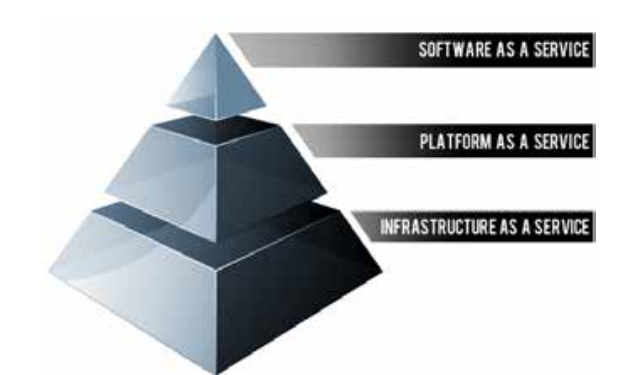
\includegraphics[width=0.65\linewidth]{Captura de pantalla 2024-10-18 211038.png}
\caption{\label{fig:cloud_computing} La pila de computación en la nube}
\end{figure}

\text{} Se analizan en detalle las tres categorías. Sin embargo, una forma muy simplificada de diferenciar estas categorías de computación en la nube es la siguiente:
\begin{itemize}
    \item Las aplicaciones \textbf{SaaS} están diseñadas para usuarios finales, entregadas a través de la web.
    \item \textbf{PaaS} es el conjunto de herramientas y servicios diseñados para hacer que la codificación y el despliegue de esas aplicaciones sean rápidos y eficientes.
    \item \textbf{IaaS} es el hardware y el software que lo potencia todo: servidores, almacenamiento, redes, sistemas operativos.
\end{itemize}


\subsection{Saas: Software como servicios}

SaaS (Software as a Service) es un modelo que permite a los consumidores utilizar aplicaciones alojadas en la nube a través de Internet, sin necesidad de gestionar la infraestructura subyacente como servidores o sistemas operativos. Los usuarios acceden a estas aplicaciones mediante navegadores web u otras interfaces. Este modelo puede basarse en suscripciones, pago por uso, o incluso ofrecerse gratuitamente con fines publicitarios. SaaS ha mostrado un rápido crecimiento y se está convirtiendo en un estándar para muchas organizaciones. Ejemplos comunes incluyen Gmail, Facebook, LinkedIn, y plataformas educativas como Moodle.

\subsubsection*{Características de SaaS}
\begin{itemize}
    \item Acceso web a software comercial.
    \item Administración centralizada del software.
    \item Modelo de “uno a muchos”.
    \item Sin gestión de actualizaciones ni parches por parte del usuario.
    \item Integración mediante APIs.
\end{itemize}

\subsubsection*{Donde SaaS no es la Mejor Opción}
\begin{itemize}
    \item Aplicaciones que requieren procesamiento rápido de datos en tiempo real.
    \item Aplicaciones que no permiten el alojamiento externo de datos por regulación.
    \item Soluciones locales que satisfacen completamente las necesidades de la organización.
\end{itemize}

\subsection{PaaS: Plataforma como Servicio}

PaaS combina la simplicidad de SaaS con el poder de IaaS, permitiendo a desarrolladores y organizaciones implementar aplicaciones en la nube. Según NIST, PaaS proporciona al consumidor la capacidad de crear o adquirir aplicaciones utilizando lenguajes de programación y herramientas compatibles con el proveedor. El consumidor controla las aplicaciones y su configuración, pero no gestiona la infraestructura subyacente, como la red, los servidores o el almacenamiento.

\subsection{PaaS: Plataforma como Servicio}

PaaS es una plataforma informática que facilita la creación de aplicaciones web de manera rápida y sin la complejidad de gestionar el software o la infraestructura subyacente. Se asemeja a SaaS, pero en lugar de entregar software, proporciona un entorno para el desarrollo de software.

\subsection*{Características de PaaS}
\begin{itemize}
    \item Servicios integrales para desarrollar y mantener aplicaciones.
    \item Herramientas web para crear y probar interfaces de usuario.
    \item Arquitectura multi-cliente para usuarios concurrentes.
    \item Escalabilidad incorporada con balanceo de carga.
    \item Integración con servicios web y bases de datos.
    \item Soporte para colaboración del equipo de desarrollo.
    \item Herramientas para gestión de facturación y suscripciones.
\end{itemize}

PaaS, similar a IaaS, se diferencia por ofrecer servicios adicionales. Generalmente, se presenta en dos enfoques: \textbf{uno como plataforma colaborativa } para el desarrollo de software, como Heroku, que soporta múltiples lenguajes; y \textbf{otro como una plataforma que utiliza datos de aplicaciones específicas}, como force.com de Salesforce, diseñada para desarrollar aplicaciones que se integren con su CRM. Ambos enfoques facilitan el desarrollo y la gestión de aplicaciones en la nube.

\subsubsection*{Dónde PaaS Tiene Sentido}

\begin{itemize}
    \item \textbf{Colaboración de Desarrolladores:} Ideal para proyectos con múltiples desarrolladores o partes externas.
    \item \textbf{Aprovechamiento de Datos Existentes:} Útil para crear aplicaciones que utilizan datos de fuentes como CRM.
    \item \textbf{Automatización de Servicios:} Permite automatizar pruebas e implementación, convirtiéndose en el enfoque dominante en el desarrollo de software.
\end{itemize}

\subsubsection*{Dónde PaaS no es la Mejor Opción}

\begin{itemize}
    \item \textbf{Portabilidad:} No es ideal si se necesita alta portabilidad del alojamiento.
    \item \textbf{Lenguajes Propietarios:} Lenguajes o enfoques que dificultan el desarrollo.
    \item \textbf{Bloqueo de Proveedor:} Dudas sobre migración si el lenguaje es propietario.
    \item \textbf{Rendimiento:} Necesidad de personalización de hardware y software para un buen rendimiento.
\end{itemize}

\subsubsection{Relación entre los Niveles de la Pila Cloud}

IaaS es la base de todos los servicios en la nube, proporcionando la infraestructura, desde hardware hasta conectividad, y ofreciendo APIs para su gestión. Sobre esta capa se construyen los servicios superiores.

PaaS se sitúa sobre IaaS, añadiendo herramientas y \textit{frameworks} para el desarrollo de aplicaciones. Incluye capacidades como bases de datos y mensajería, que facilitan a los desarrolladores la creación de aplicaciones dentro de la plataforma.

SaaS es el nivel más alto, creado a partir de IaaS y PaaS. Ofrece un entorno completo que integra aplicaciones, contenido y una experiencia de usuario, gestionado y presentado de forma accesible.

\subsection{Implementación o Despliegue}
\subsubsection{. Formatos de implementación o despliegue de los modelos de la Pila Cloud}

\subsubsection*{Nube Pública}
La nube pública es accesible al público en general y puede ser gestionada por entidades comerciales, académicas o gubernamentales. Su infraestructura está ubicada en las instalaciones del proveedor.

\subsubsection*{Nube Privada}
La nube privada es exclusiva para una organización. Puede estar gestionada por la propia organización o un tercero y se ubica dentro o fuera de las instalaciones de la empresa.

\subsubsection*{Nube Comunitaria}
La nube comunitaria es para un grupo específico de organizaciones con objetivos compartidos. Puede ser gestionada por una o varias entidades de la comunidad o por un tercero, y su infraestructura puede estar en cualquier lugar.

\subsubsection*{Nube Híbrida}
La nube híbrida combina varias formas de nubes (pública, privada o comunitaria), conectadas mediante tecnología estandarizada que permite la portabilidad de datos y aplicaciones entre ellas.

\subsection{Virtualización}

\subsubsection{Presentación}

La virtualización permite que las aplicaciones sean independientes del hardware, brindando flexibilidad para que varias aplicaciones corran en una máquina o una aplicación en varias máquinas. También facilita que los usuarios utilicen diversas plataformas (Windows, Unix, Mac) sin perder la consistencia de sus aplicaciones.

Es un elemento clave en la computación en la nube, permitiendo que los servidores creen dispositivos virtuales, lo que optimiza los recursos. Entre sus principales beneficios están:
- Reducción de costos de espacio y consumo.
- Fácil incorporación de nuevos recursos para servidores virtualizados.
- Administración simplificada y centralizada.
- Creación de entornos de prueba sin interrumpir el desarrollo.
- Aislamiento de fallos entre máquinas virtuales.

Para los proveedores de servicios en la nube, la virtualización mejora la eficiencia del hardware, permitiéndoles ofrecer productos a mejor costo. Además, beneficia a las organizaciones que pueden consolidar sus servicios internos y extenderse hacia la nube. 

\subsubsection{El hipervisor}

El hipervisor, o monitor de máquina virtual (VMM), es un software que crea, ejecuta y gestiona máquinas virtuales, aislando el sistema operativo y recursos de estas. Es fundamental en los sistemas Cloud. El hardware físico usado como hipervisor se llama "host", mientras que las máquinas virtuales son "guests". El hipervisor redistribuye los recursos como CPU, memoria y almacenamiento entre los guests o nuevas máquinas virtuales.

\subsubsection{Del hipervisor hacia los contenedores}

La virtualización basada en hipervisor crea sobrecarga de rendimiento debido a que cada máquina virtual requiere su propio sistema operativo. Para mejorar esto, surgen los contenedores, que comparten el kernel del sistema operativo host, son más ligeros y soportan mejor arquitecturas de microservicios. Son ideales para cargas de trabajo modernas como big data, IoT y edge computing en entornos de nube.

\section{Caso de Estudio}
\subsubsection*{SaaS: Caso Groupon}
Groupon, una plataforma de ofertas diarias, creció rápidamente y adoptó Zendesk como solución de ticketing para mejorar la experiencia del cliente sin sacrificar eficiencia.

\subsubsection*{PaaS: Caso Menumate}
Menumate utilizó la plataforma PaaS de Force.com para migrar aplicaciones heredadas, mejorando la gestión de licencias, soporte y otros procesos internos.

\subsubsection*{IaaS: Caso Live Smart}
Live Smart, con su programa de dietas en línea, usó Rackspace como proveedor IaaS para manejar grandes picos de tráfico, logrando una infraestructura escalable y administrada por expertos.

\section{Algunas Tecnologías Disruptivas que Operan más Eficientemente
(y necesariamente) en Cloud}
\subsection{Internet of Things (IoT)}

\subsubsection{IoT Cloud: Presentación}
La tecnología IoT permite a dispositivos de bajo poder de cómputo enviar datos continuamente, generando grandes volúmenes de información que requieren plataformas flexibles en la nube para su análisis y almacenamiento.

\subsubsection{Azure IoT Hub}
Azure IoT Hub permite la comunicación segura y confiable con miles de dispositivos, ofreciendo un back-end hospedado en la nube para conectarse a casi cualquier dispositivo.

\subsubsection{AWS IoT Device Management}
AWS IoT Device Management facilita el registro y la administración remota de dispositivos IoT, permitiendo la organización y monitoreo a gran escala para asegurar su funcionalidad.

\subsubsection{Google Cloud IoT Core}
Google Cloud IoT Core es un servicio gestionado que permite conectar, administrar e ingerir datos de dispositivos de forma segura y sencilla.

\begin{figure}[H] % 'H' forza la colocación aquí
    \centering
    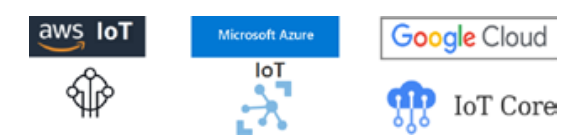
\includegraphics[width=0.65\linewidth]{Captura de pantalla 2024-10-18 230908.png}
    \caption{\label{fig:frog} Principales Plataformas IoT Cloud}
\end{figure}


\section{Enlace del repositorio}

\href{https://github.com/EvelynJazminVelazquez/SISTEMAS-DISTRIBUIDOS-ULEAM/tree/master/Computaci%C3%B3n%20en%20la%20Nube_%20Fundamentos%2C%20Cr%C3%ADticas%20y%20Desaf%C3%ADos}{Repositorio de SISTEMAS DISTRIBUIDOS de Computación en la Nube: Fundamentos,Críticas y Desafíos}


\end{document}